%=========================================================
\chapter{Modelo dinámico}	
\label{cap:modDinamico}

	Este capítulo se detallan todos los escenarios de ejecución del sistema. La figura~\ref{fig:CUcompleto1}  y la figurara~\ref{fig:CUcompleto2} muestra todos los casos de uso del sistema. En este documento solo detallamos los casos de uso del proyecto de gymnasios.

\begin{figure}[htbp]
	\begin{center}
		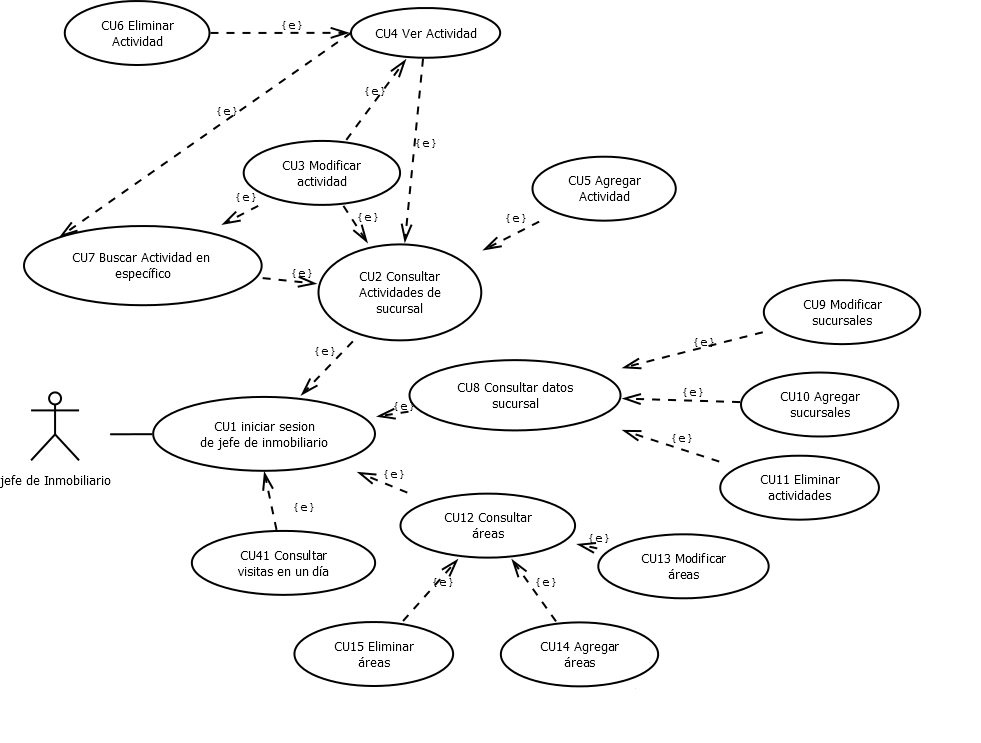
\includegraphics[angle=90, width=.7\textwidth]{images/CUcompleto1}
		\caption{Diagrama detallado del sistema parte 1.}
		\label{fig:CUcompleto1}
	\end{center}
\end{figure}

\begin{figure}[htbp]
	%\begin{center}
		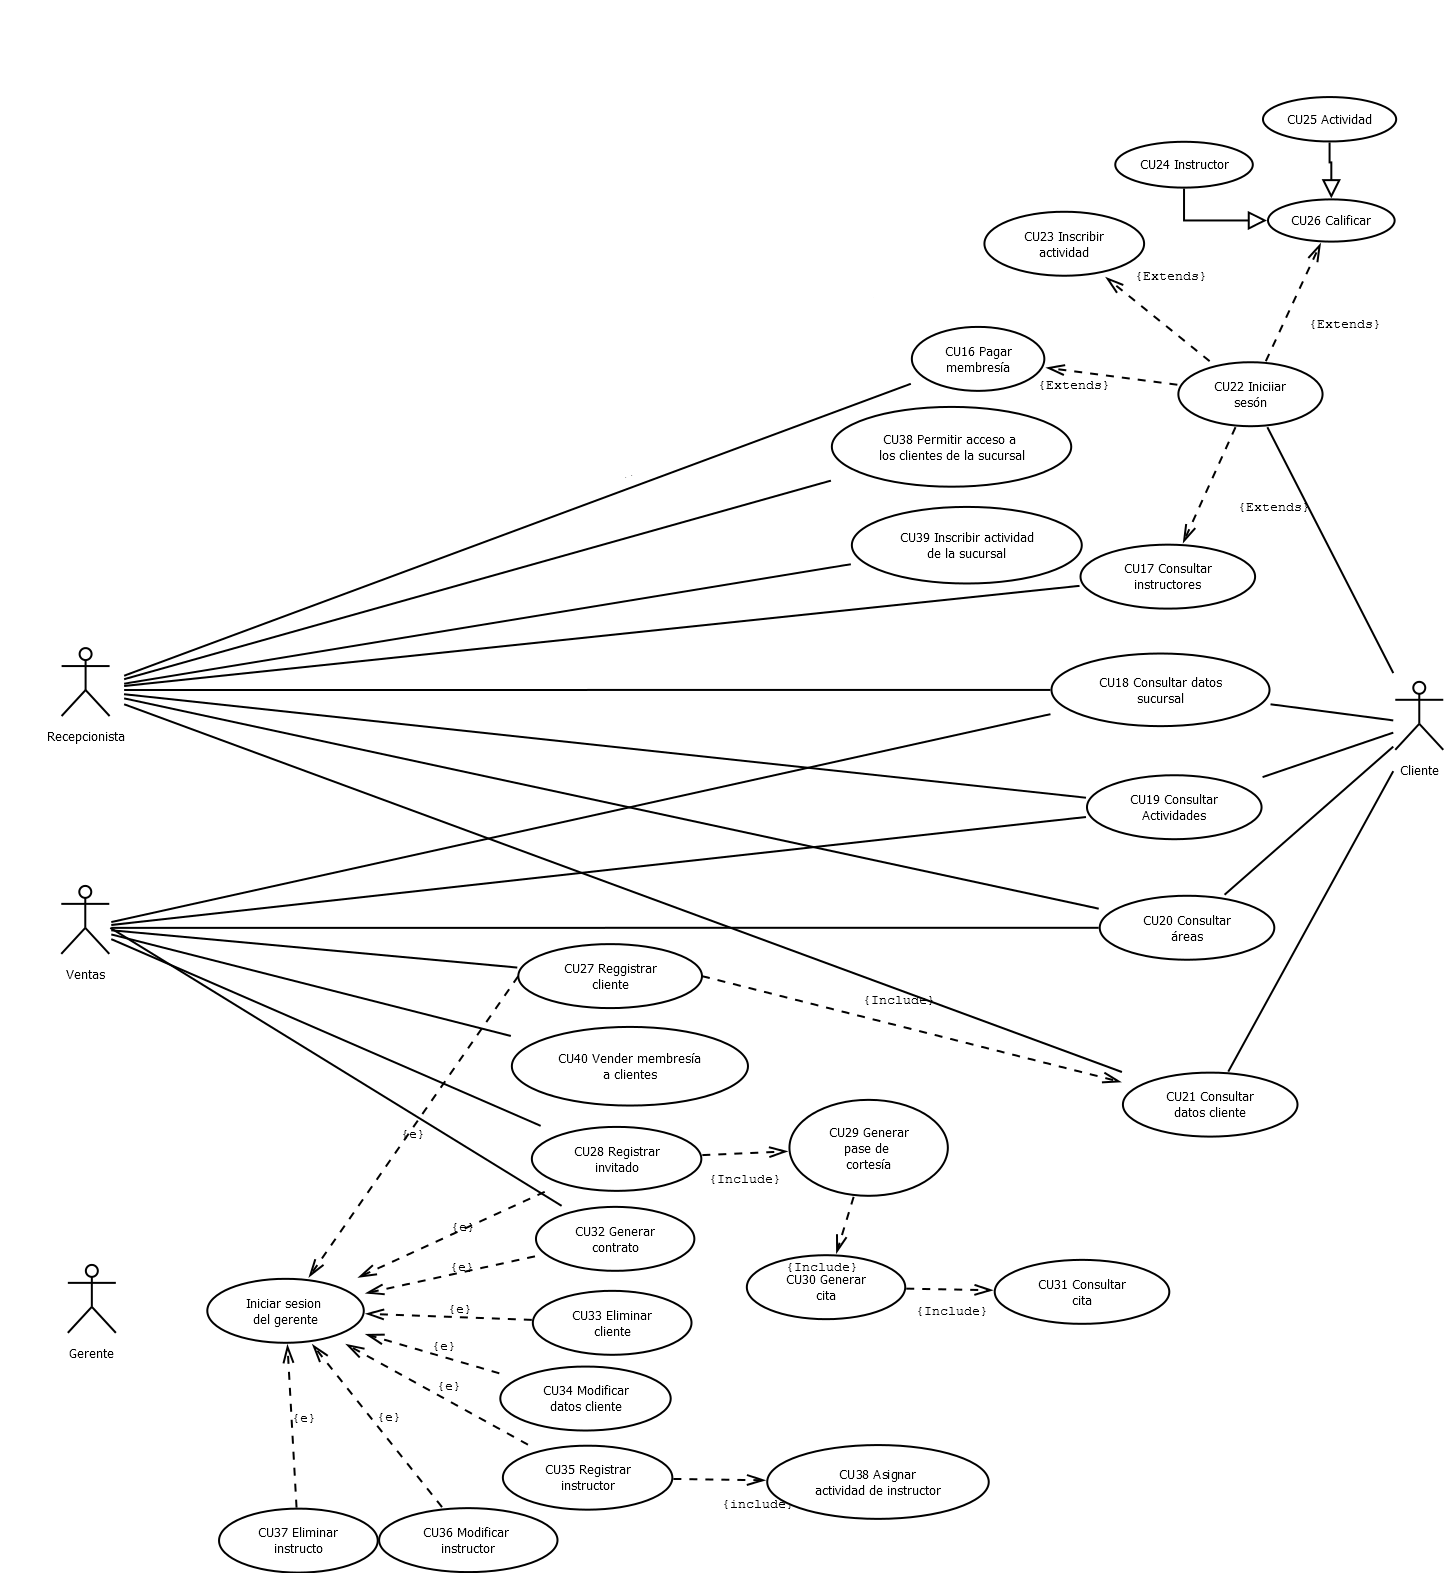
\includegraphics[angle=90, width=1.1\textwidth]{images/CUcompleto2}
		\caption{Diagrama detallado del sistema parte 1.}
		\label{fig:CUcompleto2}
	%\end{center}
\end{figure}

%---------------------------------------------------------
\section{Descripción de actores}

%---------------------------------------------------------

A continuación se detallan los casos de uso.

%---------------------------------------------------------
% CASOS DE USO

% \IUref{IUAdmPS}{Administrar Planta de Selección}
% \IUref{IUModPS}{Modificar Planta de Selección}
% \IUref{IUEliPS}{Eliminar Planta de Selección}

% 


% Copie este bloque por cada caso de uso:
%-------------------------------------- COMIENZA descripción del caso de uso.

%\begin{UseCase}[archivo de imágen]{UCX}{Nombre del Caso de uso}{
%--------------------------------------
	\begin{UseCase}{CU1}{Iniciar sesión de jefe de inmobiliario}{
	
		Validar al jefe de inmobiliario para que pueda tener acceso a la información de la sucursal, modificar o eliminar datos a través del sistema.
	}
		\UCitem{Versión}{\color{Gray}0.4}
		\UCitem{Autor}{\color{Gray}Jazmin Camarillo Martínez}
		\UCitem{Supervisa}{\color{Gray}Francisco}
		\UCitem{Actor}{Jefe de inmobiliario}
		\UCitem{Propósito}{Para que el jefe de inmobiliario sea el único que pueda realizar acciones como eliminar modificar o agregar actividades, sucursales y áreas, y mantener la información actualizada.}
		\UCitem{Entradas}{Nombre de usurario y password.}
		\UCitem{Origen}{Teclado}
		\UCitem{Salidas}{mensaje de bienvenido, nombre completo del jefe de inmobiliario, cargo del J.I. nombre de la sucursal.}
		\UCitem{Destino}{Pantalla del jefe de inmobiliario.}
		\UCitem{Precondiciones}{El jefe de inmobiliario debe estar registrado, también debe tener una cuenta correcta para poder acceder como jefe de inmobiliario y que no haya una sesión iniciada.}
		\UCitem{Postcondiciones}{El jefe de inmobiliario deberá ver un menú con; perfil, sucursales, actividades y áreas, y sus datos de salida. }
		\UCitem{Errores}{}
		\UCitem{Tipo}{Caso de uso primario}
		\UCitem{Observaciones}{}
	\end{UseCase}
%--------------------------------------
	\begin{UCtrayectoria}{Principal}
		\UCpaso[\UCactor] Introduce su Nombre de usuario y su password para poder ingresar vía la  \IUref{IU1}{Pantalla de Inicio de Sesión del Jefe de Inmobiliario.}\label{CU1LoginJI}.
		\UCpaso[\UCactor] Confirma la operación presionando el botón Iniciar Sesión.
		\UCpaso Verifica que el nombre y password son correctos para ingresar sesión del jefe de inmobiliario.
		\UCpaso Despliega la \IUref{IU2}{Pantalla inicio del jefe de inmobiliario}.
	\end{UCtrayectoria}

%--------------------------------------		
		\begin{UCtrayectoriaA}{A}{El nombre de sesión no existe}
			\UCpaso[\UCactor] Muestra el Mensaje {\bf MSG1-}``El empleado [{\em Nombre de usuario}] no existe.''.
			\UCpaso[\UCactor] Introduce nombre usuario correcto.
			\UCpaso[] Continua con el paso 3 del \UCref{CU1}.
		\end{UCtrayectoriaA}
		
%--------------------------------------
		\begin{UCtrayectoriaA}{B}{Contraseña incorrecta}
			\UCpaso Muestra el Mensaje {\bf MSG1¿2-}``El password no es correcto.''.
			\UCpaso[\UCactor] Introduce password correcto.
			\UCpaso[] Continua con el paso 3 del \UCref{CU1}.
		\end{UCtrayectoriaA}


%--------------------------------------
% Puntos de extensión
\subsection{Puntos de extensión}
\UCExtenssionPoint{
	% Cuando:
	Desea acceder a las sucursales.
	Desea acceder a las actividades.
	Desea acceder a las áreas.
	Desea acceder a su perfil.
}{
	% Durante la región:
	En el paso 5.
}{
	% Casos de uso a los que extiende:
	\hyperlink{CU2}{CU2 Consultar Actividades de sucursal}.
}
		
		
% Copie este bloque por cada caso de uso:
%-------------------------------------- COMIENZA descripción del caso de uso.

%\begin{UseCase}[archivo de imágen]{UCX}{Nombre del Caso de uso}{
%--------------------------------------
\begin{UseCase}{CU2}{Consultar Actividades de sucursal}{
		Acceder al sistema a través del inicio de sesión del jefe de inmobiliario y ver datos generales de las actividades que hay en la sucursal.
	}
	\UCitem{Versión}{\color{Gray}0.4}
	\UCitem{Autor}{\color{Gray}Jazmin Camarillo Martínez}
	\UCitem{Supervisa}{\color{Gray}Francisco}
	\UCitem{Actor}{Jefe de inmobiliario}
	\UCitem{Propósito}{Para que el jefe pueda ver las actividades que tiene la sucursal y saber si sus datos son correctos y/o poderlos modificar.}
	\UCitem{Entradas}{Botón de actividad.}
	\UCitem{Origen}{Mouse}
	\UCitem{Salidas}{Nombre de la sucursal, nombre del isntructor, hora y dia dde la actividad.}
	\UCitem{Destino}{Pantalla del jefe de inmobiliario.}
	\UCitem{Precondiciones}{El jefe de inmobiliario debe inciiar sesion para ver las actividades, debe haber al menos una actividad.}
	\UCitem{Postcondiciones}{}
	\UCitem{Errores}{}
	\UCitem{Tipo}{Caso de uso primario}
	\UCitem{Observaciones}{}
\end{UseCase}
%--------------------------------------
\begin{UCtrayectoria}{Principal}
	\UCpaso[\UCactor] Introduce su Nombre de usuario y su password para poder ingresar vía la  \IUref{IU1}{Pantalla de Inicio de Sesión del Jefe de Inmobiliario.}\label{CU1LoginJI}.
	\UCpaso[\UCactor] Confirma la operación presionando el botón Iniciar Sesión.
	\UCpaso Verifica que el nombre y password son correctos para ingresar sesión del jefe de inmobiliario.
	\UCpaso Despliega la \IUref{IU2}{Pantalla inicio del jefe de inmobiliario}.
	\UCpaso[\UCactor] Selecciona en su menú el botón de las actividades. 
	\UCpaso Despliega la \IUref{IU3}{Pantalla Actividades}.
	
\end{UCtrayectoria}


%--------------------------------------
% Puntos de extensión
\subsection{Puntos de extensión}
\UCExtenssionPoint{
	% Cuando:
	Desee ver información completa de la actividad.
	Desee editar la información.
	Desee agregar una nueva actividad.
}{
	% Durante la región:
	En el paso 5.
}{
	% Casos de uso a los que extiende:
	\hyperlink{CU3}{CU3 Modificar actividad de sucursal}.
	\hyperlink{CU4}{CU4 Ver actividad de sucursal}.
	\hyperlink{CU5}{CU5 Agregar actividad de sucursal}.
	\hyperlink{CU6}{CU6 Buscar Actividad en específico}.
}		
		


%\begin{UseCase}[archivo de imágen]{UCX}{Nombre del Caso de uso}{
%--------------------------------------
\begin{UseCase}{CU3}{Modificar actividad de sucursal}{
	Modificar los datos permitidos a través de un formulario que despliega el sistema.
	}
	\UCitem{Versión}{\color{Gray}0.4}
	\UCitem{Autor}{\color{Gray}Jazmin Camarillo Martínez}
	\UCitem{Supervisa}{\color{Gray}Francisco}
	\UCitem{Actor}{Jefe de inmobiliario}
	\UCitem{Propósito}{Para que el jefe de inmobiliario pueda mantener la informacion correcta de las actividades que hay en el sistema.}
	\UCitem{Entradas}{Nombre de la actividad, el dia y la hora que se imparte la actividad, nombre del instructor,imagen(es) y descripcion.}
	\UCitem{Origen}{Mouse y teclado}
	\UCitem{Salidas}{Numero de actividad, nombre de la actividad, nombre de la sucursal, el dia y la hora que se imparte la actividad,nombre del instructor, la descripcion de la actividad, dirección de la sucursal, imagen(es) y mensaje de operación exitosa.}
	\UCitem{Destino}{Pantalla del jefe de inmobiliario.}
	\UCitem{Precondiciones}{La actividad debe estar registrada para poder ser modificada. Debe existir en el sistema el nombre del isntructor.}
	\UCitem{Postcondiciones}{La actividad quedará modificada con los nuevos datos, si es correcto el formato con el que se lleno el formulario, la información se verá actualizada en la consulta de ver actividad.}
	\UCitem{Errores}{Formulario no este llenado de acuerdo al formato.}
	\UCitem{Tipo}{Caso de uso primario}
	\UCitem{Observaciones}{Todos los campos del formulario son obligatorios.}
\end{UseCase}
%--------------------------------------
\begin{UCtrayectoria}{Principal}
	\UCpaso[\UCactor] Selecciona en su menú el botón de las actividades vía \IUref{IU3}{Pantalla Actividades}.
	\UCpaso Despliega la \IUref{IU3}{Pantalla Actividades}.
	\UCpaso[\UCactor] Selecciona botón de Editar que aparece en la \IUref{IU3}{Pantalla Actividades}.
	\UCpaso Despliega la \IUref{IU4}{Pantalla Editar Actividad}.
	\UCpaso[\UCactor] Selecciona el recuadro que quiera modificar .
	\UCpaso[\UCactor] Borra los datos del recuadro que seleccionó para poner el nuevo dato.
	\UCpaso[\UCactor] Pulsa el botón de aceptar para confirmar la operación que se realizó.
	\UCpaso Guarda los datos que están en los recuadros.	
	\UCpaso Despliega la \IUref{IU5}{Pantalla Edición terminada}.
	\UCpaso[\UCactor] Verifica que los datos estén como el desea y oprime el botón aceptar.
	\UCpaso Despliega la \IUref{IU3}{Pantalla Actividades}.
\end{UCtrayectoria}

%\BRref{BR129}{Determinar si un Estudiante puede inscribir Seminario.} \Trayref{A}
%--------------------------------------		
\begin{UCtrayectoriaA}{A}{El jefe de inmobiliario deja información en blanco}
	\UCpaso Muestra el Mensaje {\bf MSG3-}``Todos los campos son obligatorios.''.
	\UCpaso[\UCactor] Llena los campos faltantes.
	\UCpaso[\UCactor] Continua con el paso 8 del \UCref{CU3}.
\end{UCtrayectoriaA}


% Copie este bloque por cada caso de uso:
%-------------------------------------- COMIENZA descripción del caso de uso.

%\begin{UseCase}[archivo de imágen]{UCX}{Nombre del Caso de uso}{
%--------------------------------------
\begin{UseCase}{CU4}{Ver actividad de sucursal}{
		El sistema muestrará la información completa de una actividad seleccionada.
	}
	\UCitem{Versión}{\color{Gray}0.4}
	\UCitem{Autor}{\color{Gray}Jazmin Camarillo Martínez}
	\UCitem{Supervisa}{\color{Gray}Francisco}
	\UCitem{Actor}{Jefe de inmobiliario}
	\UCitem{Propósito}{Para que el jefe de inmobiliario pueda revisar que los datos de la actividad sean correctos.}
	\UCitem{Entradas}{botón de ver actividad.}
	\UCitem{Origen}{Teclado}
	\UCitem{Salidas}{Numero de actividad, nombre de la actividad, nombre de la sucursal, el dia y la hora que se imparte la actividad,nombre del instructor, la descripcion de la actividad, dirección de la sucursal, imagen(es).}
	\UCitem{Destino}{Pantalla del jefe de inmobiliario.}
	\UCitem{Precondiciones}{El jefe de inmobiliario debe estar dentro de susesión para poder ver la información. La actividad que desee ver, debe estar registrada.}
	\UCitem{Postcondiciones}{}
	\UCitem{Errores}{Actividad inexistente}
	\UCitem{Tipo}{Caso de uso primario}
	\UCitem{Observaciones}{}
\end{UseCase}
%--------------------------------------
\begin{UCtrayectoria}{Principal}
	\UCpaso[\UCactor] Ingresa a la \IUref{IU3}{Pantalla de Actividades.}\label{CU1LoginJI}.
	\UCpaso[\UCactor] Oprime el botón de ver.
	\UCpaso Despliega la \IUref{IU6}{Pantalla Ver Actividad}.
	\UCpaso Oprime el botón de aceptar para regresar a la  \IUref{IU3}{Pantalla de Actividades.}\label{CU1LoginJI}.
\end{UCtrayectoria}


%--------------------------------------
% Puntos de extensión
\subsection{Puntos de extensión}
\UCExtenssionPoint{
	% Cuando:
	Desea modificar datos de actividad.
}{
	% Durante la región:
	En el paso 3.
}{
	% Casos de uso a los que extiende:
	\hyperlink{CU3}{CU3 Modificar actividad de sucursal}.
}



% Copie este bloque por cada caso de uso:
%-------------------------------------- COMIENZA descripción del caso de uso.

%\begin{UseCase}[archivo de imágen]{UCX}{Nombre del Caso de uso}{
%--------------------------------------
\begin{UseCase}{CU5}{Agregar actividad a la sucursal}{
		El Jefe de inmobiliario podrá agregar una nueva actividad al sistema.
	}
	\UCitem{Versión}{\color{Gray}0.4}
	\UCitem{Autor}{\color{Gray}Jazmin Camarillo Martínez}
	\UCitem{Supervisa}{\color{Gray}Francisco}
	\UCitem{Actor}{Jefe de inmobiliario}
	\UCitem{Propósito}{Para que cada que se agregue una nueva actividad a la sucursal se pueda incorporar su información al sistema.}
	\UCitem{Entradas}{}
	\UCitem{Origen}{Teclado}
	\UCitem{Salidas}{.}
	\UCitem{Destino}{Pantalla del jefe de inmobiliario.}
	\UCitem{Precondiciones}{.}
	\UCitem{Postcondiciones}{El jefe de inmobiliario deberá ver un menú con; perfil, sucursales, actividades y áreas, y sus datos de salida. }
	\UCitem{Errores}{}
	\UCitem{Tipo}{Caso de uso primario}
	\UCitem{Observaciones}{}
\end{UseCase}
%--------------------------------------
\begin{UCtrayectoria}{Principal}
	\UCpaso[\UCactor] Introduce su Nombre de usuario y su password para poder ingresar vía la  \IUref{IU1}{Pantalla de Inicio de Sesión del Jefe de Inmobiliario.}\label{CU1LoginJI}.
	\UCpaso[\UCactor] Confirma la operación presionando el botón Iniciar Sesión.
	\UCpaso Verifica que el nombre y password son correctos para ingresar sesión del jefe de inmobiliario.
	\UCpaso Despliega la \IUref{IU2}{Pantalla inicio del jefe de inmobiliario}.
\end{UCtrayectoria}

%--------------------------------------		
\begin{UCtrayectoriaA}{A}{El nombre de sesión no existe}
	\UCpaso[\UCactor] Muestra el Mensaje {\bf MSG1-}``El empleado [{\em Nombre de sesión}] no existe.''.
	\UCpaso[\UCactor] Introduce nombre usuario correcto.
	\UCpaso[] Continua con el paso 3 del \UCref{CU1}.
\end{UCtrayectoriaA}

%--------------------------------------
\begin{UCtrayectoriaA}{B}{Contraseña incorrecta}
	\UCpaso Muestra el Mensaje {\bf MSG12-}``El password no es correcto.''.
	\UCpaso[\UCactor] Introduce password correcto.
	\UCpaso[] Continua con el paso 3 del \UCref{CU1}.
\end{UCtrayectoriaA}


%--------------------------------------
% Puntos de extensión
\subsection{Puntos de extensión}
\UCExtenssionPoint{
	% Cuando:
	Desea acceder a las sucursales.
	Desea acceder a las actividades.
	Desea acceder a las áreas.
	Desea acceder a su perfil.
}{
	% Durante la región:
	En el paso 5.
}{
	% Casos de uso a los que extiende:
	\hyperlink{CU2}{CU2 Consultar Actividades de sucursal}.
}

% \IUref{IUAdmPS}{Administrar Planta de Selección}
% \IUref{IUModPS}{Modificar Planta de Selección}
% \IUref{IUEliPS}{Eliminar Planta de Selección}

% 


% Copie este bloque por cada caso de uso:

%-------------------------------------- COMIENZA descripción del caso de uso.


%-------------------------------------- COMIENZA descripción del caso de uso.

%\begin{UseCase}[archivo de imágen]{CUX}{Nombre del Caso de uso}{
%--------------------------------------
	\begin{UseCase}{CU22}{Iniciar sesión cliente gimnasio}{
		Permite  al cliente del gimnasio autenticarse en el sistema mediante correo y su contraseña para poder ingresar a su cuenta.
	}
		\UCitem{Versión}{\color{Gray}0.2}
		\UCitem{Autor}{\color{Gray}Daniel.}
		\UCitem{Supervisa}{\color{Gray}Luis.}
		\UCitem{Actor}{\hyperlink{Cliente}{Cliente}}
		\UCitem{Propósito}{Que el cliente pueda pueda acceder a su información, actividades que tiene inscritas o para poder inscribir alguna y ver sus instructores.}
		\UCitem{Entradas}{Correo electrónico, contraseña}
		\UCitem{Origen}{El actor mediante el teclado ingresara los datos mencionados}
		\UCitem{Salidas}{Nombre completo, Dirección, Calle, No. int, No. Ext. Col. Del./Mun. C.P, Peso, Enfermedades, Alergias, Tipo de sangre, Medicamentos.}
		\UCitem{Destino}{Pantalla del cliente.}
		\UCitem{Precondiciones}{Que el cliente este registrado en el sistema, que no haya una sesión ya activa.}
		\UCitem{Postcondiciones}{El cliente va ver su pantalla de inicio.}
		\UCitem{Errores}{Que el correo sea incorrecto, que la contraseña sea errónea, que no este registrado.}
		\UCitem{Tipo}{Caso de uso primario}
		\UCitem{Observaciones}{Este caso de uso tendrá pestañas adicionales para ver sus actividades, horarios e instructores que tiene a demás de poder inscribir actividad. A grandes rasgos este C.U. solo muestra los datos personales del cliente del gimnasio.}
	\end{UseCase}
%--------------------------------------

	\begin{UCtrayectoria}{Principal}
		\UCpaso[\UCactor] Ingresa su correo.  %\IUref{IU23}{Pantalla de Control de Acceso}\label{CU17Login}.
		\UCpaso[\UCactor] Ingresa su contraseña.%\BRref{BR129}{Determinar si un Estudiante puede inscribir Seminario.} \Trayref{A}.
		\UCpaso[\UCactor] Da clic en el botón de iniciar sesión\Trayref{A}\label{CU15ValidarQR}.  %\IUref{IU32}{Pantalla de Selección de Seminario}
		\UCpaso valida que el usuario y contraseña son correctas para iniciar sesión. 
		\UCpaso mostrara el nombre completo, su direccion y los datos medicos..% \BRref{BR130}{Determinar si un Estudiante puede inscribirse en un Seminario} \Trayref{C}.
		\UCpaso  mostrara en el menu superior el nombre del usuario y una lista deplegable ahi mismo con la opción de ver cursos, ver instructores y cerrrar sesión.\Trayref{C}\label{CU15RealizarPago}. %\BRref{BR143}{Validar el horario del estudiante} \Trayref{D}.		
	\end{UCtrayectoria}

%--------------------------------------		


%--------------------------------------
% Puntos de extensión
%\subsection{Puntos de extensión}
%\UCExtenssionPoint{
	% Cuando:
%	Desea conocer las materias cursadas.
%}{
	% Durante la región:
%	Del paso 4 al paso 9.
%}{
	% Casos de uso a los que extiende:
%	\hyperlink{CU3.4}{CU3.4 Consultar historial académico}.
%}
		
		
		
%-------------------------------------- TERMINA descripción del caso de uso.


%-------------------------------------- COMIENZA descripción del caso de uso.

%\begin{UseCase}[archivo de imágen]{UCX}{Nombre del Caso de uso}{
%--------------------------------------
	\begin{UseCase}{CU23}{Inscribir actividad}{
		Permite  al cliente poder inscribirse en una actividad que se imparte en una sucursal.
	}
		\UCitem{Versión}{\color{Gray}0.1}
		\UCitem{Autor}{\color{Gray}Daniel}
		\UCitem{Supervisa}{\color{Gray}Luis}
		\UCitem{Actor}{\hyperlink{Cliente}{Cliente}}
		\UCitem{Propósito}{Que el usuario pueda ir a la actividad sin que le nieguen el acceso y conozca el horario en el que debe asistir.}
		\UCitem{Entradas}{Nombre Actividad, Sucursal, horario}
		\UCitem{Origen}{Teclado}
		\UCitem{Salidas}{Mensaje,Nombre Actividad,Sucursal,horario}
		\UCitem{Destino}{Pantalla del cliente}
		\UCitem{Precondiciones}{ Que el cliente haya iniciado sesión, que exista la actividades que se desea inscribir, que haya cupo en la actividad deseada.}
		\UCitem{Postcondiciones}{El cliente vera la actividad inscrita en su lista de actividades.}
		\UCitem{Errores}{No haya cupo en la actividad por inscribir}
		\UCitem{Observaciones}{}
	\end{UseCase}
%--------------------------------------
	\begin{UCtrayectoria}{Principal}
		\UCpaso[\UCactor] Desde la pantalla donde termina el CU22 seleccionar el botón de inscribir actividad.
		\UCpaso Muestra la pantalla de inscribir actividad.
		\UCpaso Muestra los campos que se deberán llenar para inscribir la actividad.
		\UCpaso[\UCactor] llena los campos y dar clic en inscribir.
		\UCpaso[\UCactor] confirma la operación oprimiendo el botón de aceptar. 
		\UCpaso Valida que la actividad y el horario que el usuario eligió exista.
		\UCpaso Valida que haya cupo en la actividad que eligió el usuario.
		\UCpaso Despliega msg3 "Actividad inscrita".
		\UCpaso Muestra la pantalla de inicio de cliente.	
	\end{UCtrayectoria}
%-------------------------------------- TERMINA descripción del caso de uso.


%-------------------------------------- COMIENZA descripción del caso de uso.

%\begin{UseCase}[archivo de imágen]{UCX}{Nombre del Caso de uso}{
%--------------------------------------
\begin{UseCase}{CU25}{Calificar Actividad.}{
		El cliente selecciona una puntuación para la actividad en un intervalo del 1 al 5 y se quedara guardada.
	}
	\UCitem{Versión}{\color{Gray}0.1}
	\UCitem{Autor}{\color{Gray}Daniel}
	\UCitem{Supervisa}{\color{Gray}Luis}
	\UCitem{Actor}{\hyperlink{Cliente}{Cliente}}
	\UCitem{Propósito}{ Que el cliente pueda transmitir una retro alimentación para el gimnasio y que pueda tener un mejor servicio. }
	\UCitem{Entradas}{Nombre Actividad, Calificación, Comentario }
	\UCitem{Origen}{Mouse y teclado.}
	\UCitem{Salidas}{Mensaje, Calificación}
	\UCitem{Destino}{Pantalla del cliente}
	\UCitem{Precondiciones}{ Que el cliente haya iniciado sesión, que este inscrito a alguna actividad.}
	\UCitem{Postcondiciones}{Que el cliente no este inscrito en la actividad que quiere calificar,que no exista la actividad que quiere calificar el cliente, que el cliente califique fuera del rango permitido.}
	\UCitem{Errores}{}
	\UCitem{Observaciones}{}
\end{UseCase}
%--------------------------------------

\begin{UCtrayectoria}{Principal}
	\UCpaso[\UCactor] Desde la pantalla donde termina el CU22 seleccionar el botón de Actividades.
	\UCpaso[\UCactor] Selecciona el botón de calificar actividad.
	\UCpaso Despliega los campos a llenar para calificar una actividad en la misma pantalla.
	\UCpaso[\UCactor] Selecciona una actividad
	\UCpaso[\UCactor] Asigna una calificación y un comentario que sera de manera opcional.
	\UCpaso[\UCactor] Confirma la operación oprimiendo el botón de "aceptar"..
	\UCpaso Valida que la actividad que seleccionó el usuario exista y que este inscrito en esa actividad.
	\UCpaso Mustra MSG4 "Calificación hecha" y la calificación de la actividad.
	
\end{UCtrayectoria}

<<<<<<< HEAD
%-------------------------------------- TERMINA descripción del caso de uso.

=======
<<<<<<< HEAD
%-------------------------------------- TERMINA descripción del caso de uso.
=======
e%-------------------------------------- TERMINA descripción del caso de uso.
>>>>>>> 0eff6495fec5e6e8df531b40918ac1ccee0f67e3
>>>>>>> 4435e9eea844c41d312547d202b75a2558a68b41



%\begin{figure}[htbp]
%	\begin{center}
%		\includegraphics[width=.8\textwidth]{images/vistas/buscarcliente}
%		\caption{Buscar cliente}
%		\label{fig:Ventas}
%	\end{center}
%\end{figure}

\section{Guión de Pruebas}

\subsection{Guión de prueba 1}
\begin{itemize}
\item ID: Guión 01
\item ALCANCE: CU01
\item NOMBRE: Iniciar sesioón de jefe de inmobiliario  
\item PREPARACIÓN:\\
-En la BD debe de estar registrado el jefe de inmobiliario.
\item CP 1:
\item DATOS DE ENTRADA:\\
	\begin{itemize}
		\item Correo electrónico del J.I: Jefe\_inmobiliario\@hotmail.com
		\item Contraseña: SOY\_elJefe1
	\end{itemize}
\begin{center}			
	\begin{tabular}{|l|l|l|l|}
		\hline
		CP 1\\
		PASOS\\
		\hline 1.- Ingresar a la pantalla IU08\\
		\hline 2.- Introducir el numero de cliente.\\
		\hline 3.- Presionar el botón buscar\\
		\hline
	\end{tabular}
\end{center}
\item SALIDAS: Verificación y resultado si tiene acceso permitido el usuario a las diferentes 
áreas del gimnasio.
\item CP 2:
\item DATOS DE ENTRADA:\\
-numero de empleado: 354\\
\begin{center}			
	\begin{tabular}{|l|l|l|l|}
		\hline
		CP 2\\
		PASOS\\
		\hline 1.- Ingresar a la pantalla IU08\\
		\hline 2.- Introducir el numero de cliente.\\
		\hline 3.- Presionar el botón buscar\\
		\hline
	\end{tabular}
\end{center}
\item SALIDAS: Verificación y resultado si tiene acceso permitido el usuario a las diferentes 
\item CP 3:
\item DATOS DE ENTRADA:\\
-numero de cliente: -123\\
\begin{center}			
	\begin{tabular}{|l|l|l|l|}
		\hline
		CP 3\\
		PASOS\\
		\hline 1.- Ingresar a la pantalla IU08\\
		\hline 2.- Introducir el numero de cliente.\\
		\hline 3.- Presionar el botón buscar\\
		\hline
	\end{tabular}
\end{center}
\item SALIDAS: "Sin especificar".
\item CP 4:
\item DATOS DE ENTRADA:\\
-numero de cliente: 500\\
\begin{center}			
	\begin{tabular}{|l|l|l|l|}
		\hline
		CP 4\\
		PASOS\\
		\hline 1.- Ingresar a la pantalla IU08\\
		\hline 2.- Introducir el numero de cliente.\\
		\hline 3.- Presionar el botón buscar\\
		\hline
	\end{tabular}
\end{center}
\item SALIDAS: Muestra una pantalla con un formulario de datos a llenar del cliente.
\end{itemize}

%---------------------------------------------------------
% PANTALLAS DE LOS CASOS DE USO
\IUfig[.5]{LoginJI}{IU1}{Pantalla de login del jefe de inmobiliario.}

\IUfig[.5]{inicioSesion}{IU2}{Pantalla de Inicio de Sesión del jefe de inmobiliario.}

\IUfig[.5]{ActividadesJI}{IU3}{Pantalla de Actividades.}

\IUfig[.5]{EditarActividad}{IU4}{Pantalla de Editar Actividad.}

\IUfig[.5]{FinEditarAC}{IU5}{Pantalla de Edición terminada.}

\IUfig[.5]{VerActividadJI}{IU6}{Pantalla de Ver Actividad.}

\IUfig[.5]{loginCliente}{IU22}{Pantalla de Inicio de sesion del cliente.}

\IUfig[.5]{inicioCliente}{IU23}{Pantalla de Inicio del cliente.}



